%% Template for Master thesis
%% ===========================
%%
%% You need at least KomaScript v3.0.0,
%% e.g. available in Texlive 2009
\documentclass  [
  paper    = a4,
  BCOR     = 10mm,
  twoside,
  fontsize = 12pt,
  fleqn,
  toc      = bibnumbered,
  toc      = listofnumbered,
  numbers  = noendperiod,
  headings = normal,
  listof   = leveldown,
  version  = 3.03
]                                       {scrreprt}

% used pagages
\usepackage     [utf8]                  {inputenc}
\usepackage     [T1]                    {fontenc}
\usepackage                             {color}
\usepackage                             {amsmath}
\usepackage                             {graphicx}
\usepackage     [english]               {babel}
\usepackage                             {natbib}
\usepackage                             {hyperref}

% my packages
\usepackage{bm}
\usepackage{subcaption}

% links
\definecolor{darkblue}{rgb}{0.0,0.0,0.4}
\definecolor{darkgreen}{rgb}{0.0,0.4,0.0}
\hypersetup{
    colorlinks,
    linkcolor=black,
    citecolor=darkgreen,
    urlcolor=darkblue
}

\begin{document}
  %% title pages similar to providet template instead of maketitle
  %% Titelseiten ähnlich zum Layout des Formulars von der
%% Fakultät für Physik und Astronomie
%%
%% Weitere Infos:
%% http://www.physik.uni-heidelberg.de/aktuelles/studium/
%% (PDF link: ...studium/download/145/Vorlage_Diplomarbeit_Formular.pdf)

%% Titelintro
\thispagestyle{empty}
\begin{center}
  \renewcommand{\baselinestretch}{2.00}
  \Large\sffamily
  Fakult\"{a}t f\"{u}r Physik und Astronomie\\
  \large
  Ruprecht-Karls-Universit\"{a}t Heidelberg
  \par\vfill\normalfont
  Masterarbeit\\
  Im Studiengang Physik\\
  vorgelegt von\\
  Martin Huber\\
  geboren in Frankenthal (Pfalz)\\
  2019\\
\end{center}
\newpage

%% Titelseite
\thispagestyle{empty}
\begin{center}
  \renewcommand{\baselinestretch}{2.00}
  \Large\bfseries\sffamily
    Implementierung und Fusion von \\
    modellprädiktiver Regelung mit \\
    neuronalen Netzwerken zur \\ 
    autonomen Navigation von humanoiden Robotern
  \par
  \vfill
  \large\normalfont
  Die Masterarbeit wurde von Martin Huber\\
  ausgeführt am\\
  Institut für Optimierung, Robotik und Biomechanik\\
  unter der Betreuung von\\
  Frau Prof. Katja Mombaur
  %% Bei externen Masterarbeiten hier noch den zweiten Betreuer einfügen
  %% und den vspace in Z. 45 entsprechend reduzieren
\end{center}\par
\vspace{5\baselineskip}

% Zeilenabstand zurücksetzen
\renewcommand{\baselinestretch}{1.00}\normalsize % select either german
  %% this will generate title pages similar to the template provided
%% by the Department of Physics and Astronomy Heidelberg
%%
%% More information:
%% http://www.physik.uni-heidelberg.de/aktuelles/studium/
%% (PDF link: ...studium/download/145/Vorlage_Diplomarbeit_Formular.pdf)

%% Titleintro
\thispagestyle{empty}
\begin{center}
  \renewcommand{\baselinestretch}{2.00}
  \Large\sffamily
  Department of Physics and Astronomy\\
  \large University of Heidelberg
  \par\vfill\normalfont
  Master thesis\\
  in Physics\\
  submitted by\\
  (name and surname)\\
  born in (place of birth)\\
  (year of submission)
\end{center}
\newpage

%% Titlepage
\thispagestyle{empty}
\begin{center}
  \renewcommand{\baselinestretch}{2.00}
  \Large\bfseries\sffamily
    (Title)\\
    (of)\\
    (Master thesis)
  \par
  \vfill
  \large\normalfont
  This Master thesis has been carried out by (Name Surname)\\
  at the\\
  (institute)\\
  under the supervision of\\
  (Frau/Herrn Prof./Priv.-Doz. Name Surname)
  %% additionally insert second supervisor here if carrying out an
  %% external diploma thesis. Reduce vspace in L. 44 accordingly.
\end{center}\par
\vspace{5\baselineskip}

% reset baselinestretch
\renewcommand{\baselinestretch}{1.00}\normalsize % or english title page
  %% Abstract page
%% =============
%%
%% Content of abstract pages has been put into seperate pages to simplify
%% word counting. Use e.g. the unix command
%%   wc abstract-ger.tex
%% or
%%   wc abstract-eng.tex
%% to get the number of words contained in these files.
\thispagestyle{empty}
\begin{center}
  \begin{minipage}[c][0.48\textheight][b]{0.9\textwidth}
    \small
    \textbf{
      Verhaltensklonung zur autonomen Navigation humanoider Roboter mit Nichlinearer Modellprädiktiver Regelung:
    }\par
    \vspace{\baselineskip}
    In dieser Arbeit erkunden wir die Möglichkeiten der Verhaltensklonung zur autonomen Navigation humanoider Roboter durch bloße Bilder. Hierfür wird eine nichtlineare, Modellprädiktive Regelung, die es ermöglicht, stabile Lauftrajektorien in Echtzeit zu erzeugen, implementiert und evaluiert. Es wird demonstriert, dass minimale Veränderung in der Bildverarbeitung genügen, um vielseitige Bewegungsstrategien in vielfältigen dynamischen und statischen Umgebungen zu erlernen. Diese Einfachheit der Lösung wird als passende Ergänzung zur Meidung von Konvexen Hindernissen identifiziert, welche durch Randbedingungen die Lösungen der nichtlinearen Modellprädiktiven Regelung einschränken. Alle Experimente werden an Heicub, einer Variente des iCub, durchgeführt, welcher speziell für Optimalsteuerung in der Fortbewegung am Istituto Italiano di Tecnologiia in Genove entwickelt wurde. Die Auswertung von Stabilitätskriterien zeigt weiterhin, dass ein menschlicher Kontrolleur, einem künstlichen Agenten gegenüber, nicht überlegen ist. Um die präsentierte Methode schließlich auf tauschende Aufgaben zu erweitern, vereinfachen wir die wechselnden Umgebungen auf ein gut gelöstes Klassifizierungsproblem.
  \end{minipage}\par
  \vfill
  \begin{minipage}[c][0.48\textheight][b]{0.9\textwidth}
    \small
    \textbf{
      Behavioral Cloning for Autonomous Navigation of Humanoid Robots with Nonlinear Model Predictive Control:
    }\par
    \vspace{\baselineskip}
    In this work, we investigate the capabilities of behavioral cloning for autonomous navigation of humanoid robots from raw image input. Therefore, a nonlinear model predictive control that allows for real-time generation of stable walking trajectories is implemented and evaluated. It is demonstrated that minor modifications in the vision pipeline are sufficient for the learning of versatile motion strategies in various dynamic and static environments. This simplicity is identified as a well-suited addition to the avoidance of convex obstacles, which are represented by constraints to the solution of the implemented nonlinear model predictive control. All of the experiments are carried out on Heicub, a descendant of the iCub, which was specially designed for optimal control in locomotion at the Istituto Italiano di Tecnologia in Genova. The evaluation of balance criteria further reveals that there is no superiority of a human controller over an artificial agent. Finally, we investigate on reinforcement learning methods to replace the behavioral cloning by self-taught policies.

  \end{minipage}
\end{center}


  \tableofcontents
  
  %% chapters
  \chapter{Introduction}
  % humanoids (icub, others), problem statement, research aim and objectives
    
  \chapter{State of the Art}
  \label{sec::2_sota}
  % contributions
    
  \chapter{Background}
  To generate dynamically balanced walking trajectories for humanoid robots and to let them navigate the environment autonomously, there are several posed challenges that we need to cover. As the logical starting point, in section \ref{sec::31_hm} - Humanoid Walking, we want to address the real time generation of walking trajectories for humanoid robots first, and then think of ways to replace the human user by an artificial agent in the control loop. As discussed in section \ref{sec::2_sota} - State of The Art, there are several ways to achieve this, but of particular interest to us are novel methods that evolved from the toolbox of machine learning techniques. Center to these new methods will be neural nets that we will try to train on solving the task of autonomous navigation in different ways, as shown in section \ref{sec::32_ml} - Machine Learning.
\begin{figure}[h]
	\centering
	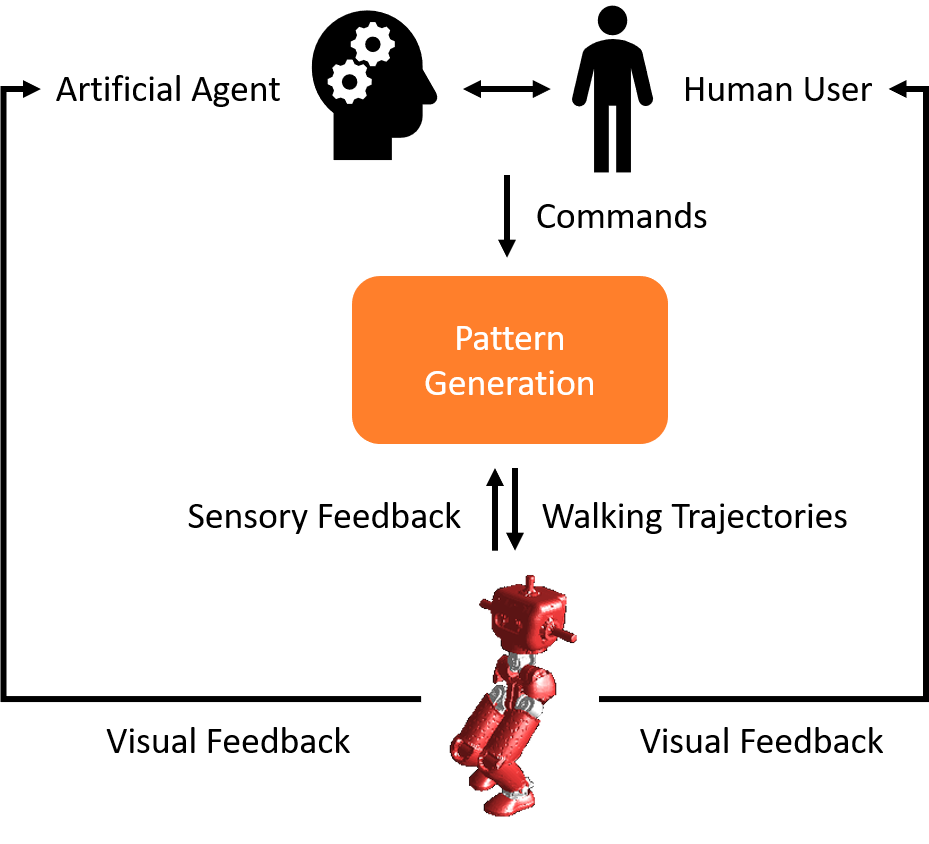
\includegraphics[scale=.5]{chapters/03_background/img/control_loop.png}
	\caption{\label{fig::3_cl} Proposed control loop to navigate the robot with either a human user or an artificial agent.}
\end{figure}   % introduction to background
  \section{Humanoid Walking}
\label{sec::31_hw}
To get started with and to understand the presented concepts that generate dynamically balanced walking trajectories, we shall have a look at figure \ref{fig::3_cl} once more. The pattern generation therein (orange box), consists of four main building blocks: Forward kinematics, nonlinear model predictive control (NMPC), interpolation, and inverse kinematics. The relation between these four building blocks is shown in fig. \ref{fig::31_pg}.
\begin{figure}[h]
	\centering
	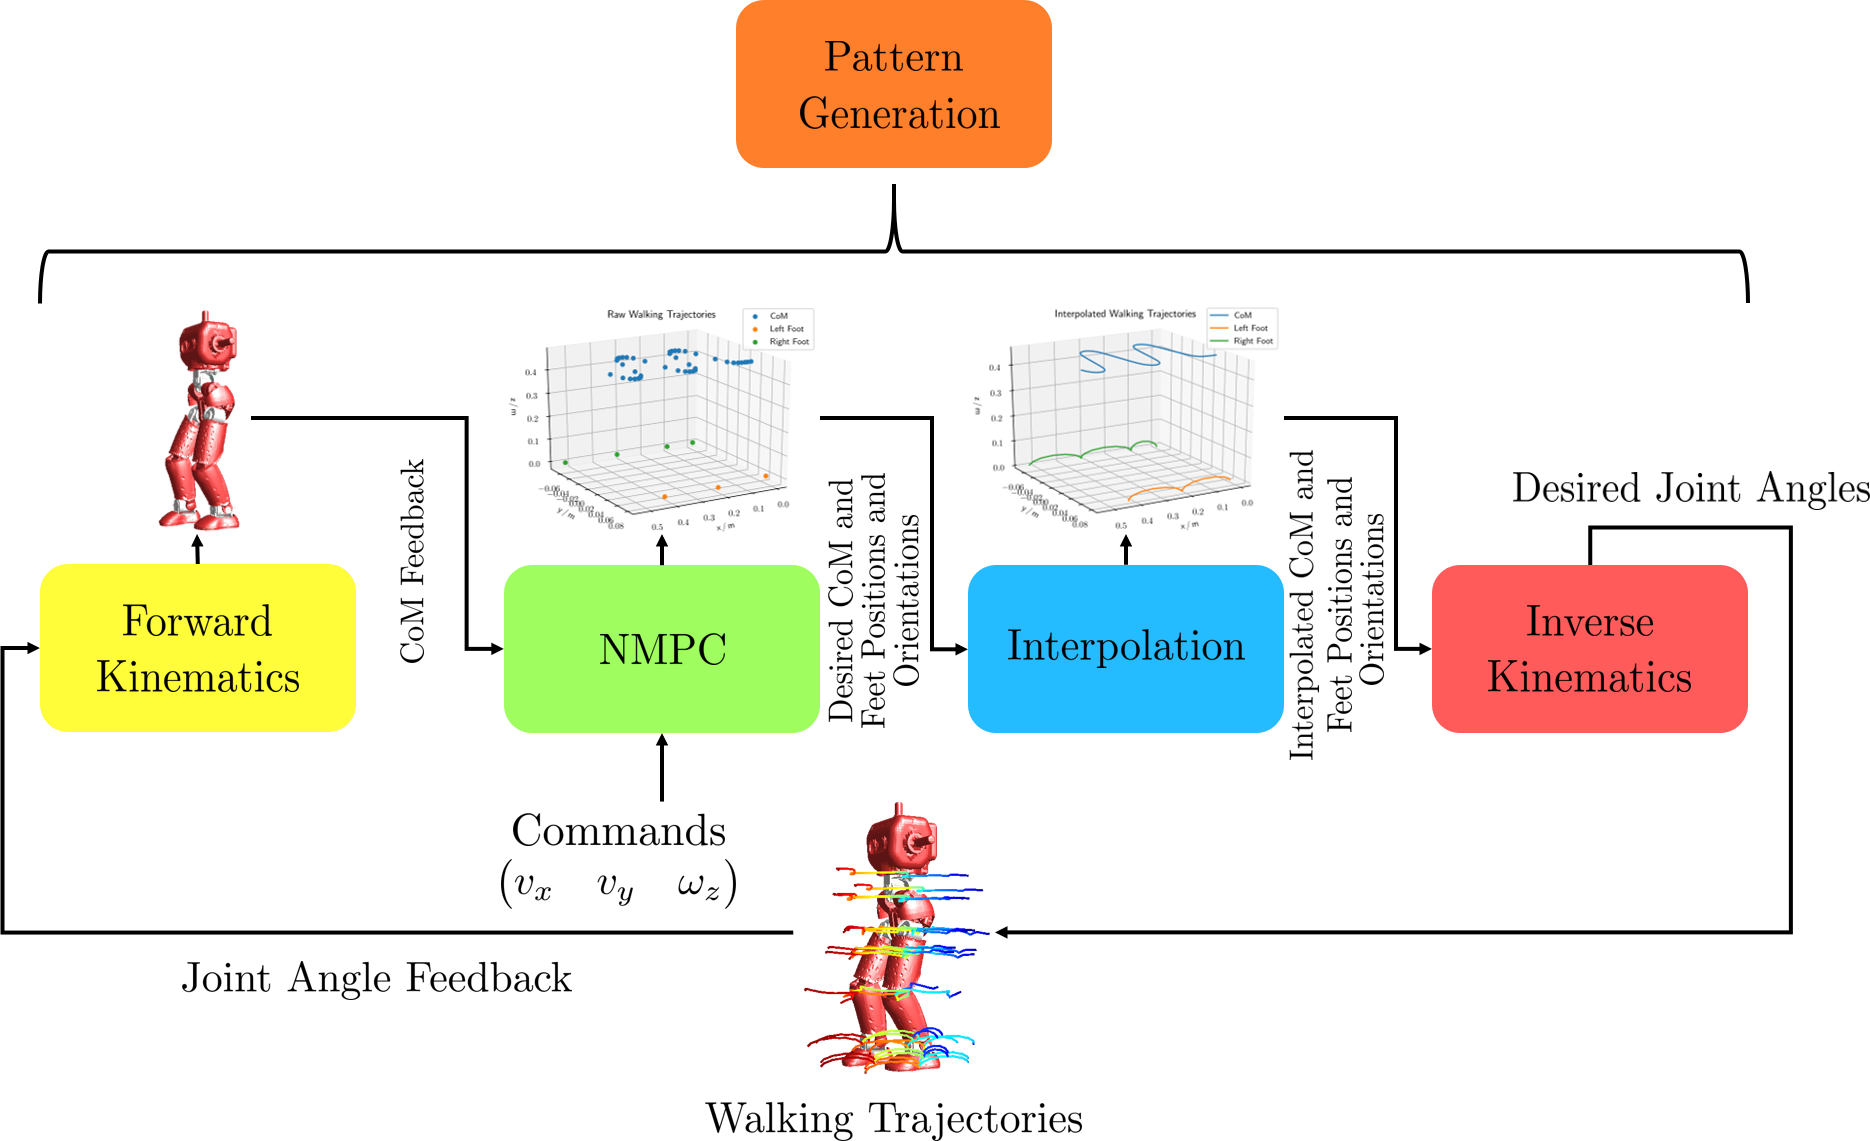
\includegraphics[scale=.5]{chapters/03_background/img/pattern_generation.png}
	\caption{Building blocks of the pattern generation. To understand the greater picture, a connection can be drawn to fig. \ref{fig::3_cl}, where the orange box represents the one shown in this figure.}
	\label{fig::31_pg}
\end{figure}
The natural entry point, to this otherwise closed control loop, is given by the commands that enter the nonlinear model predictive control. Commands are passed in the form of a desired velocity $\mathbf{v}_\text{ref}$ that the robot's center of mass (CoM) shall satisfy optimally according to a cost function that also takes dynamic balance and a smooth motion into account. The future desired positions and orientations for the CoM and the feet then result from the solution to a sequentially quadratic problem that tries to minimize this cost function. The balance criteria within this problem formulation is based upon the zero moment point (ZMP) around which the whole control framework is built. It is only by simplifying the robot's model that we can solve the optimal control problem in real time. Therefore, we assume the robot to be a linear inverted pendulum, for which we have a well defined analytical relation between the CoM and the ZMP. The minimization of the distance between the analytical expression of the ZMP and the foot placement results in the desired dynamic balance. As shown in fig. \ref{fig::31_pg}, the desired CoM and the feet positions and orientation, as they are obtained from the NMPC, are sparsely distributed in space. Moreover, there is neither information about how the feet shall move along the z-axis, nor along the x-, and y-axis, but only where they should be placed in the x-y-plane. Therefore, as the subsequent step to the NMPC, we need to add an interpolation. The interpolation interpolates the trajectories of the CoM to obtain a finer sampling time. Additionally, the movement of the feet in the x-, y-, and z-direction, as well as their orientation, is computed by polynomials that we require to satisfy the initial and end conditions of the foot placement. Put together, the nonlinear model predictive control and the interpolation between the resulting subsequent solutions for the positions and orientation of both, the CoM and the feet, describe dynamically balanced trajectories, given that the humanoid robot of interest resembles the physics of an inverted pendulum. Now to bridge the gap between dynamically balanced trajectories in Cartesian space, and a humanoid robot that actually satisfies them with its CoM and its feet, the inverse kinematics problem needs to be addressed. The inverse kinematics, which follow immediately after the interpolation step, take the positions and orientations of the CoM and the feet as constraints and find a composite of joint angles that fulfill them. The continuity of subsequent solutions is therein assured by initializing the inverse kinematics with the previous solution. Resulting joint angles, once passed to the humanoid, then result in walking trajectories, as indicated in fig. \ref{fig::31_pg} by the colored lines at the joints of the robot. Due to the inherent mismatch of the robot's physics from that of an inverted pendulum, as well as other effect like friction, there is a chance that the desired joint angles differ from the actually achieved ones. To compensate for the discrepancy, the last building block of the pattern generation is the feedback of the measured CoM to the NMPC. The CoM is computed by reading out the achieved joint angles, so that the forward kinematics can be utilized to determine the positions and orientations of the humanoid's links in space, and therefore the CoM.
\\\\
As already highlighted in the previous paragraph, special attention has to be given to the zero moment point, since it defines the central concept of the presented pattern generation. We therefore will explain its theoretical foundations, as well as its analytical relationship to the CoM for simplified physical models, and ways to measure it with force torque sensors in the section that lies ahead - Zero Moment Point.





    % short overview of humanoid walking
  \subsection{Zero Moment Point}
\label{sec::311_zmp}
The key metric in this work, for the generation of a dynamically balanced gait, is the zero moment point. The concept was first introduced by Miomir Vukobratovi\'{c} and Davor Juri\v{c}i\'{c} in 1968 \cite{vukobratovic1968contribution}\cite{vukobratovic1969contribution} and first utilized 1984 to generate walking trajectories for the WL-10RD robot \cite{yamaguchi1993development}. The most intuitive understanding for the ZMP arises by thinking about the realization of the simplest arbitrary possible walking motion for which a humanoid robot will not fall. This motion is achieved by ensuring the feet's whole area, and not only the edge, is in contact with the ground \cite{vukobratovic2004zero}, or put in other words, we require the robot not to rotate about its feet edges. This constraint can be met by having a reaction force $\bm{F}_r$ between the foot and the ground, which compensates for all external moments $\bm{M}_x$, and $\bm{M}_y$ around the x-, and y-axis at any time (fig. \ref{fig::311_zmp}).
\begin{figure}[h]
	\centering
	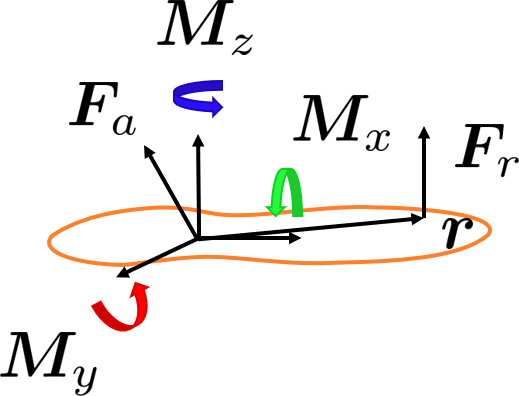
\includegraphics[scale=.5]{chapters/03_background/img/zero_moment_point.png}
	\caption{Forces acting on the sole.}
	\label{fig::311_zmp}
\end{figure}
The point $\bm{r}$, at which the reaction force acts, is physically only meaningful if it lies within the support polygon of the foot. Not only can it not exist outside of the support polygon, since there was no point of interaction between the foot and the ground then, but also was the robot to overturn under these circumstances. Therefore, the ZMP is defined as that point on the ground at which the net moment of the inertial forces has no component along the horizontal axes \cite{hirai1998development}\cite{dasgupta1999making}. We now came to appreciate the importance of the support polygon for the definition of the zero moment point. 
\begin{figure}[h]
	\centering
	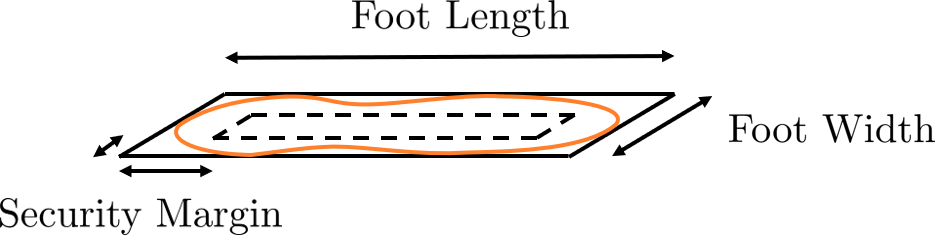
\includegraphics[scale=.5]{chapters/03_background/img/support_polygon.png}
	\caption{Full support polygon, and the resulting support polygon with security margin (dashed lines).}
	\label{fig::311_support_polygon}
\end{figure}
The support polygon is defined as the convex hull of all contact points of the feet with the ground, so the minimal number of points to fully contain all of them. As the most restrictive case for balance, in this work we will only consider the support polygon of one foot at a time. Since the convex hull of a foot is well described by a rectangle, we only rely on the foot width (\href{https://github.com/mhubii/nmpc_pattern_generator/blob/bc79a6d4f9bcfd3794146355af44429f5b7a9fe0/libs/pattern_generator/configs.yaml#L14}{link}), and foot length (\href{https://github.com/mhubii/nmpc_pattern_generator/blob/bc79a6d4f9bcfd3794146355af44429f5b7a9fe0/libs/pattern_generator/configs.yaml#L15}{link}) to fully describe it. Also, to ensure that the zero moment point never comes close to the edges of the feet and therefore to provide balance, we define a security margin to their boarders (\href{https://github.com/mhubii/nmpc_pattern_generator/blob/bc79a6d4f9bcfd3794146355af44429f5b7a9fe0/libs/pattern_generator/configs.yaml#L3}{link}). The respective values are robot specific and can be set in the configurations file by following the provided links.
\\\\
As already pointed out, within this work, we will use a simplified physical model of the humanoid solve the optimal control problem in real time. We will deal with this approximation in the following paragraph - Zero Moment Point of a Linear Inverted Pendulum.
\subsubsection{Zero Moment Point of a Linear Inverted Pendulum}
Dynamically balanced walking trajectories can be generated by simplifying the dynamics of humanoid robots to those of a linear inverted pendulum \cite{kajita2003biped}. A rigorous derivation for the analytic relation between the center of mass and the zero moment point of a linear inverted pendulum can be found in \cite{kajita2014introduction}, but for the sake of simplicity we rather explain the physics in terms of cutting forces, for which a short introduction can be found in the summary of the lecture Robotics 1 (\href{https://drive.google.com/file/d/1aN1ujXTOlHzO2kLPK7TQRkWfdY-pGzUF/view}{link}). 
\begin{figure}[h]
	\centering
	\subcaptionbox{}%
	[.4\linewidth]{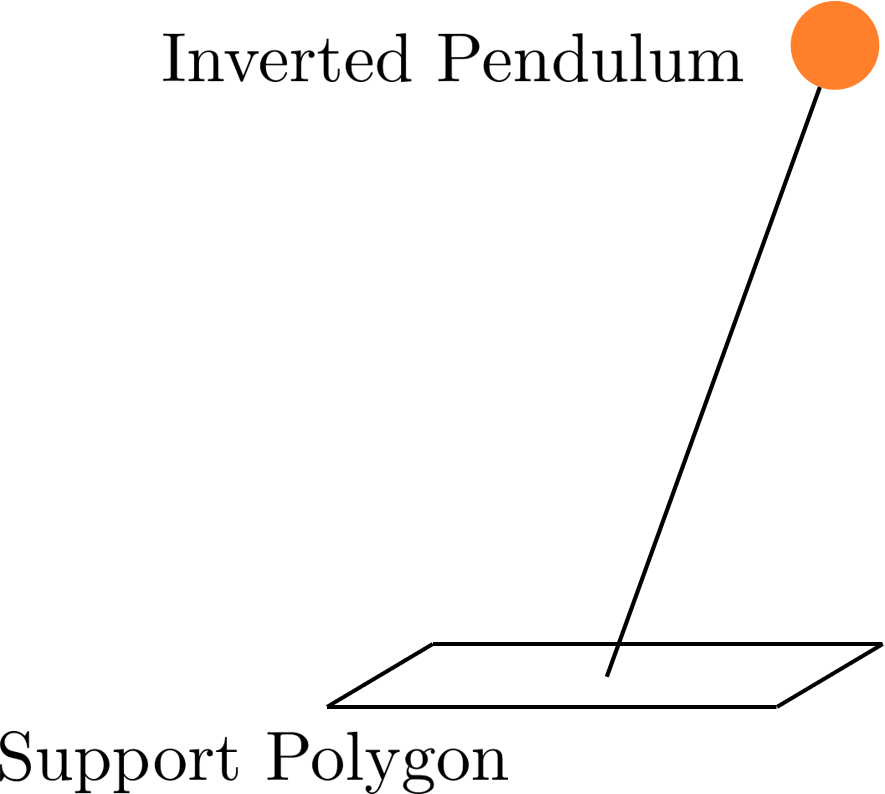
\includegraphics[scale=.3]{chapters/03_background/img/inverted_pendulum.png}}
	\subcaptionbox{}%
	[.4\linewidth]{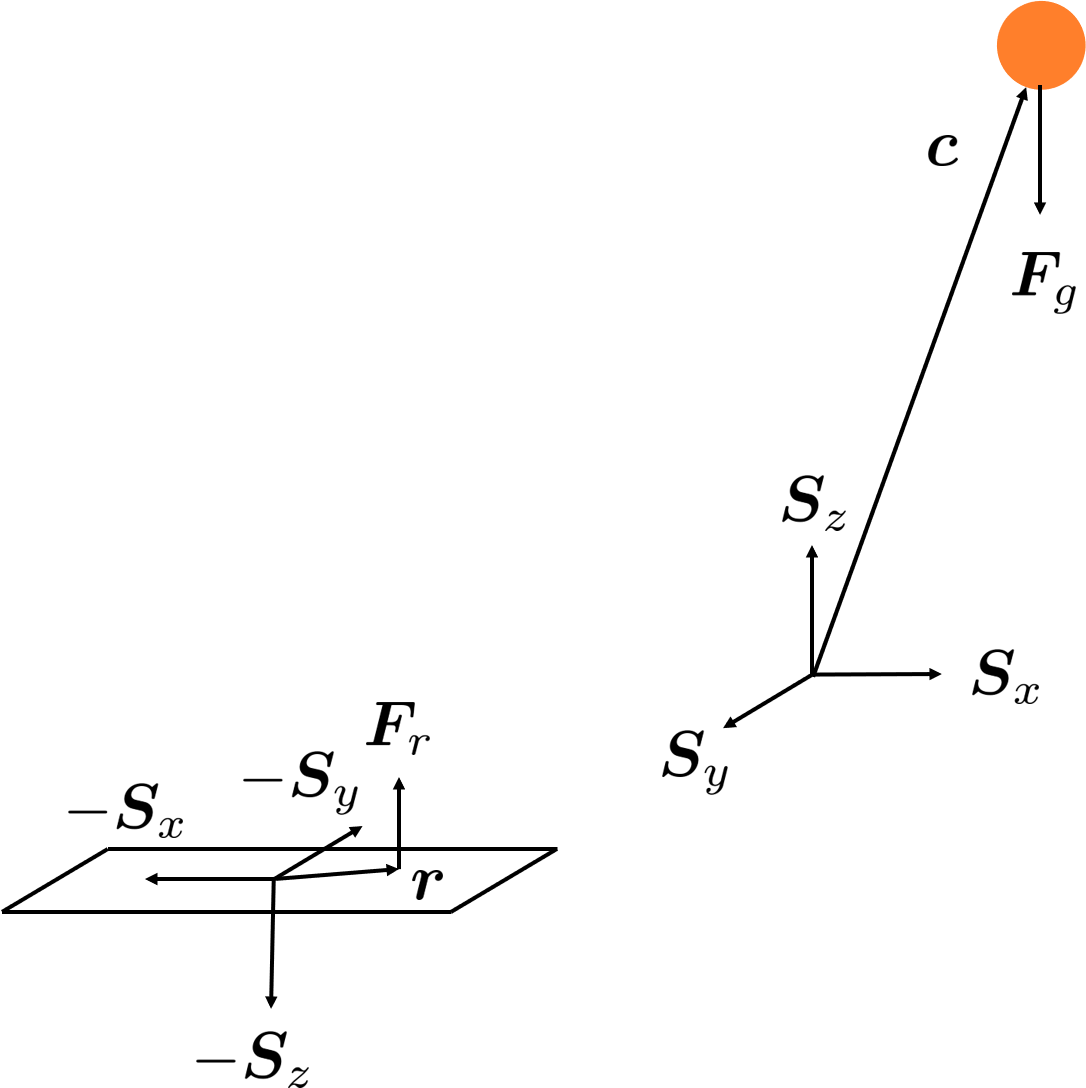
\includegraphics[scale=.3]{chapters/03_background/img/inverted_pendulum_free_body_diagram.png}}
	\caption{Linear inverted pendulum with a support polygon (a), and the corresponding free body diagram with cutting forces $\bm{S}_{x/y/z}$ (b).}
	\label{fig::311_lip}
\end{figure}
The system of interest is shorty depicted in figure \ref{fig::311_lip}. We assume the support polygon of the shown linear inverted pendulum to have zero mass. By introducing cutting forces $\bm{S}_{x/y/z}$ for each degree of freedom in which the motion of the linear inverted pendulum is restricted, we obtain the free body diagram (fig. \ref{fig::311_lip}), for which the acting forces are
\begin{align}
	m\ddot{\bm{c}} &=\quad\bm{S} - \bm{F}_g 
	\label{eq::311_pendulum_force} \\
	\bm{0} &= -\bm{S}+\bm{F}_r
	\label{eq::311_support_polygon_force}
\end{align}
where $\bm{S}=\bm{S}_x+\bm{S}_y+\bm{S}_z$. The respective moments, since we do not take any inertias into account, are given by
\begin{align}
	\bm{0} &= (\bm{0}-\bm{c})\times\bm{S} + \bm{M} 
	\label{eq::311_pendulum_moment}\\	
	\bm{0} &= (\bm{r}-\bm{0})\times\bm{F}_r - \bm{M}
	\label{eq::311_support_polygon_moment}	
\end{align}
where the transfer of the moment $\bm{M}$ may for example be induced by friction. If we replace $\bm{S}=\bm{F}_r$ from eq. \ref{eq::311_support_polygon_force}, equations \ref{eq::311_pendulum_moment} and \ref{eq::311_support_polygon_moment} yield 
\begin{align}
	\bm{0} = (\bm{r}-\bm{c})\times\bm{S} = \begin{pmatrix}
	\quad(r_y - c_y)S_z - (r_z - c_z)S_y \\
	-(r_x - c_x)S_z + (r_z - c_z)S_x \\
	\quad(r_x - c_x)S_y - (r_y - c_y)S_x
	\end{pmatrix}
	\label{eq::311_momentum_transfer}
\end{align}
Since our goal is to have a robot that does not fall, we want to achieve that the acceleration along the z-axis becomes zero, hence $\ddot{c}_z=0$. Given this assumption, we can infer from eq. \ref{eq::311_pendulum_force} that $S_z=mg$, as well as $S_x = \ddot{c}_xm$, and $S_y = \ddot{c}_ym$. Furthermore, our foot shall not lift off the floor, and therefore we have $r_z=0$. If we take these assumptions and plug them into the first to rows of eq. \ref{eq::311_momentum_transfer}, we find
\begin{align}
	r_x &= c_x - c_z\frac{\ddot{c}_x}{g}\\
	r_y &= c_y - c_z\frac{\ddot{c}_y}{g}
	\label{eq::311_zmp}
\end{align}
Therein, $r_x$, and $r_y$ are the x-, and y-coordinates of the zero moment point, given the assumption of a linear inverted pendulum. We can see that the position if dependent on the height of the point mass, which is in turn dependent on the robot. The specific values can be set in the configurations file (\href{https://github.com/mhubii/nmpc_pattern_generator/blob/bc79a6d4f9bcfd3794146355af44429f5b7a9fe0/libs/pattern_generator/configs.yaml#L27}{link}).
\\\\
We have now found a simple analytic expression for the relationship of the zero moment point and the center of mass, which will help us to formulate an optimal control problem that we can solve in real time. This simplification is of course only true to some extend, and we need to find a way to verify its accuracy. The easiest way to do so is to measure the real zero moment point. We will further elaborate on this within the next paragraph - Measurement of the Zero Moment Point, and we will derive a method that only relies on force torque sensors in the ankle.
\subsubsection{Measurement of the Zero Moment Point}
There are several methods that enable us to measure the position of the zero moment point, among them the utilization of pressure sensitive soles, as outlined in \cite{kajita2014introduction}. Furthermore, there exist approximate approaches that involve the knowledge of all acting external forces \cite{huang2001planning}, which can for example be obtained from unconstrained inverse dynamics \cite{michel2017dynamic}. Since we can rely on measurements of force torque sensors that are located at the ankles, we will infer the position of the zero moment point from them \cite{kajita2014introduction}. If we consider the force torque sensor to be located a position $\bm{p}_i$ (fig. \ref{fig::311_force_torque}), then we can obtain the moment about any point $\bm{p}$ according to eq. \ref{eq::311_moment}.
\begin{align}
	\bm{\tau}(\bm{p}) = (\bm{p}_i-\bm{p})\times \bm{f}_i + \bm{\tau}_i
	\label{eq::311_moment}
\end{align}
by definition, the moment about the zero moment point vanishes along the horizontal axes, therefore we can then set $\tau_x = \tau_y = 0$ in eq. \ref{eq::311_moment} and then solve for the position to obtain the zero moment point (eq. \ref{eq::311_x_pos_zmp} and \ref{eq::311_y_pos_zmp}).
\begin{align}
	p_x &= \frac{\left[-\tau_{i,y}-(p_{i,z}-p_z)f_{i,x}+p_{i,x}f_{i,z}\right]}{f_{i,z}}
	\label{eq::311_x_pos_zmp}\\
	p_y &= \frac{\left[-\tau_{i,x}-(p_{i,z}-p_z)f_{i,y}+p_{i,y}f_{i,z}\right]}{f_{i,z}}
	\label{eq::311_y_pos_zmp}
\end{align}
If we further choose our coordinate system to lie along the z-axis of the force torque sensor (fig. ...), we can simplify equations \ref{eq::311_x_pos_zmp} and \ref{eq::311_y_pos_zmp} to find
\begin{align}
	p_x &= \frac{(-\tau_{i,y}-f_{1,x}d)}{f_{1,z}} 
	\label{eq::311_x_pos_zmp_simp}\\
	p_y &= \frac{(\tau_{i,x}-f_{1,y}d)}{f_{1,z}}
	\label{eq::311_y_pos_zmp_simp}
\end{align}
We can use equations \ref{eq::311_x_pos_zmp_simp} and \ref{eq::311_y_pos_zmp_simp} to determine the position of the zero moment point for the left and the right foot with respect to coordinates frames that are attached to the respective foot. These circumstances change once not only one, but both feet are in contact with the ground. What still holds true, in the case of a dynamically balanced gait, is the fact that the positions which we just obtained from equations \ref{eq::311_x_pos_zmp_simp} and \ref{eq::311_y_pos_zmp_simp} represent points where the interaction of the robot with the environment can solely be described by a single force along the z-axis. All other forces or torques cancel out. Therefore, to determine the position of the zero moment point for the double support phase, we need to modify equation \ref{eq::311_moment} slightly. This yields 
\begin{align}
	\bm{\tau}(\bm{p}) = \sum_{i\in\{L, R\}} (\bm{p}_i - \bm{p})\times\bm{f}_i
	\label{eq::311_moment_ds}
\end{align}
where the individual torques are now zero and the only forces $\bm{f}_i$ that exist between the robot and the environment can be described by the z-component which are measured at the ankles' force torque sensors. Yet again, to obtain the position of the zero moment point, we have to set the x-, and y-components of the torque in equation \ref{eq::311_moment_ds} to zero and find
\begin{align}
	p_x &= \frac{\sum_{i\in\{L, R\}}p_{i,x}f_{i,z}}{\sum_{i\in\{L, R\}}f_{i,z}} \\
	p_y &= \frac{\sum_{i\in\{L, R\}}p_{i,y}f_{i,z}}{\sum_{i\in\{L, R\}}f_{i,z}}
\end{align}
These expressions of course only hold true in a shared coordinate system and therefore we need to transform the position of the zero moment point which we obtained from equations \ref{eq::311_x_pos_zmp_simp} and \ref{eq::311_y_pos_zmp_simp} to the world frame. Finally, we can write down the formulation for the zero moment point which holds equally true for the single and double support phase
\begin{align}
	p_x &= \frac{p_{R,x}f_{R,z}+p_{L,x}f_{L,z}}{f_{R,z}+f_{L,z}}  \\
	p_y &= \frac{p_{R,y}f_{R,z}+p_{L,y}f_{L,z}}{f_{R,z}+f_{L,z}}
\end{align}
At this point we are now equipped with a general understanding for the zero moment point, as well as with the knowledge of simplified models to compute it analytically, and a method to measure it so that we can evaluate the performance of a potential pattern generator which is based upon the zero moment point. Therefore, in the next chapter - Nonlinear Model Predictive Control, we will try to understand a method that allows us to generate dynamically balanced center of mass and feet trajectories, which 
  % zero moment point
  \subsection{Nonlinear Model Predictive Control}
\label{sec::312_nmpc}
At the heart of nonlinear model predictive control stands sequential quadratic programming. Before we come to the actual problem formulation, we need to understand how sequential quadratic programming can be used to solve nonlinear optimization problems. We will then come to recognize that if we can find a canonical formulation of our problem, it will become possible to apply sequential quadratic programming to it. The next paragraph - Sequential Quadratic Programming, will therefore shortly introduce the reader to the desired method that will be used to solve the  nonlinear optimization problem, while the subsequent paragraph - Canonical Formulation of Nonlinear Model Predictive Control, will then explain how to fit humanoid walking into this framework.
\subsubsection{Sequential Quadratic Programming}
Sequential quadratic programming is a powerful concept to solve nonlinearly constrained optimization problems. The nonlinear programming problem to be solved is of the form
\begin{align}
	\min_{\bm{x}}\, &f(\bm{x})\\
	\text{subject to: } &\bm{h}(\bm{x}) = \bm{0}\\
	&\bm{g}(\bm{x}) \leq \bm{0},
\end{align}
where $f:\,\mathcal{R}^N\rightarrow\mathcal{R}$, $\bm{h}:\,\mathcal{R}^N\rightarrow\mathcal{R}^M$, and $\bm{g}:\,\mathcal{R}^N\rightarrow\mathcal{R}^P$ \cite{boggs1995sequential}. These problems arise in a variety of applications in science and include quadratic problems as special cases. The great strength of sequential quadratic programming is its ability to solve problems with nonlinear constraints, and its basic idea is to model nonlinear programming at an approximate solution $\bm{x}_k$ by a quadratic subproblem, so to find a solution to this subproblem, in order to construct a better approximation $\bm{x}_{k+1}$. Now given an objective function $f(\bm{x})$ represents a sum of squares, the problem at hand turns into a nonlinear least squares problem, and the minimization can be expressed in terms of a Gauss-Newton method \cite{schittkowski1988solving}. That is, given an objective function $f(\bm{x}) = \frac{1}{2}\bm{F}(\bm{x})^T\bm{F}(\bm{x})$, where $\bm{F}=\left(f_1,...,f_l\right)^T$, we can apply a quasi Gauss-Newton method as follows
\begin{align}
	\nabla^2f(\bm{x})\Delta\bm{x} + \nabla f(\bm{x}) = 0,
	\label{eq::312_quasi_gn}
\end{align}
where the gradient and the Hessian matrix are given as
\begin{align}
	\nabla f(\bm{x}) &= \nabla \bm{F}(\bm{x})\bm{F}(\bm{x}) \\
	\nabla^2 f(\bm{x}) &= \nabla \bm{F}(\bm{x})\nabla\bm{F}(\bm{x})^T + \bm{B}(\bm{x}).
\end{align}
Therein, $\bm{B}(\bm{x}) = \sum_1^lf_i(\bm{x})\nabla^2f_i(\bm{x})$. If we are now sufficiently close to an optimal solution $\bm{x}^*$, such that $\bm{F}(\bm{x}^*) = \left(f_1(\bm{x}^*),...,f_l(\bm{x}^*)\right)^T=\bm{0}$, we can neglect $\bm{B}(\bm{x^*})$, which turns equation \ref{eq::312_quasi_gn} into the previously stated Gauss-Newton minimization problem
\begin{align}
	\min_{\Delta\bm{x}}\,||\nabla\bm{F}(\bm{x_k})^T\Delta\bm{x}+\bm{F}(\bm{x}_k)||,
\end{align}
where a new iterate is obtained by $\bm{x}_{k+1}=\bm{x}_k + \alpha_k\Delta \bm{x}$ with an appropriate step length parameter $\alpha_k$. The presented approach assures quadratic convergence, when starting sufficiently close to an optimal solution. Within the next section, we will understand how to apply this concept to control the zero moment point of a linear inverted pendulum in a balanced manner.
\subsubsection{Canonical Formulation of Nonlinear Model Predictive Control}
\cite{kajita2003biped} % original mpc
\cite{herdt2010online} % herdt
\cite{herdt2010walking} % walking without thinking
\cite{naveau2016reactive} % nmpc % nonlinear model predictive control
  \subsection{Interpolating Trajectories}
\label{sec::313_it}
As already shortly depicted in figure \ref{fig::31_pg}, we need to interpolate the trajectories that we obtain from the nonlinear model predictive control. This especially holds true for the feet, since the computed results do only consider the pendulums dynamic balance with respect to the x-, and the y-position, but not with respect to a robot that has to lift its feet along the z-axis. Furthermore, the feet's movement shall be executed such they stop moving when they are about to touch the ground. This constraint, and others, will be achieved by interpolating the feet trajectories with polynomials. In order to then match the center of mass trajectory's temporal resolution with the feet trajectories', we will upscale it under the already well known assumption of a linear inverted pendulum. The resulting trajectories are shown in figure \ref{fig::313_ip}, and will further be explained in the following. 
\begin{figure}[h]
	\centering
	\subcaptionbox{}%
	[.4\linewidth]{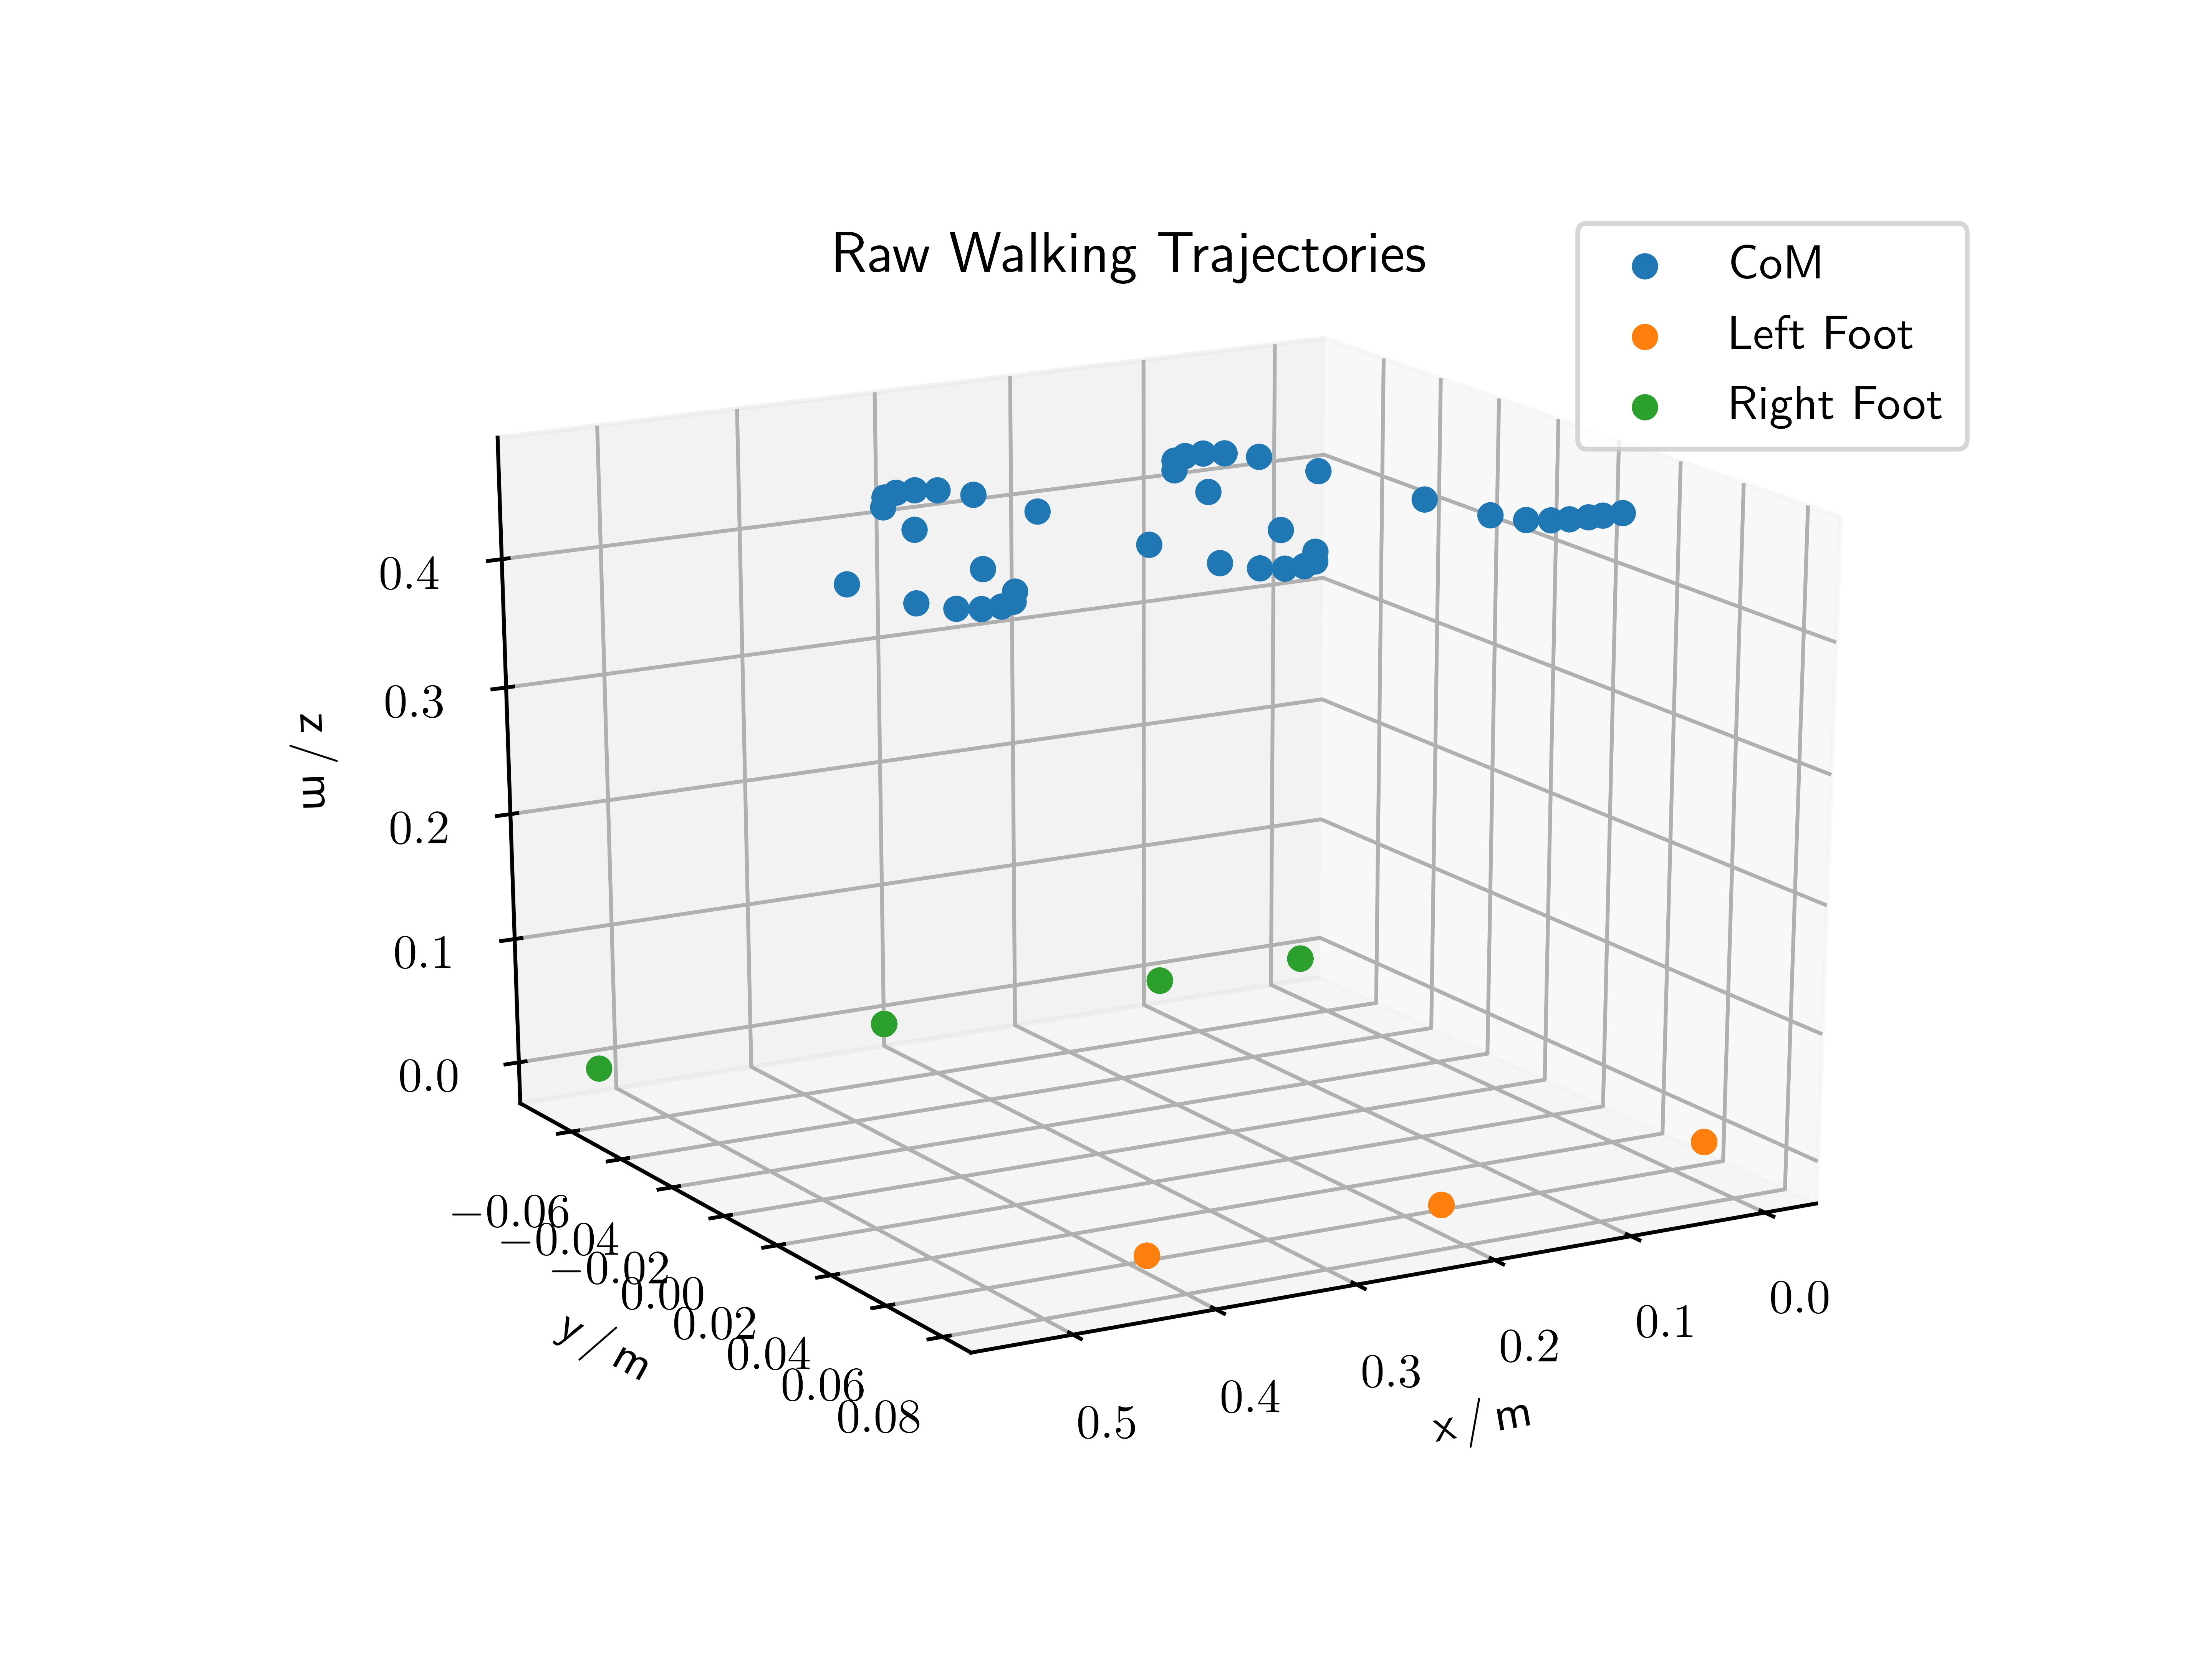
\includegraphics[scale=.4]{chapters/03_background/img/raw_results.png}}
	\subcaptionbox{}%
	[.4\linewidth]{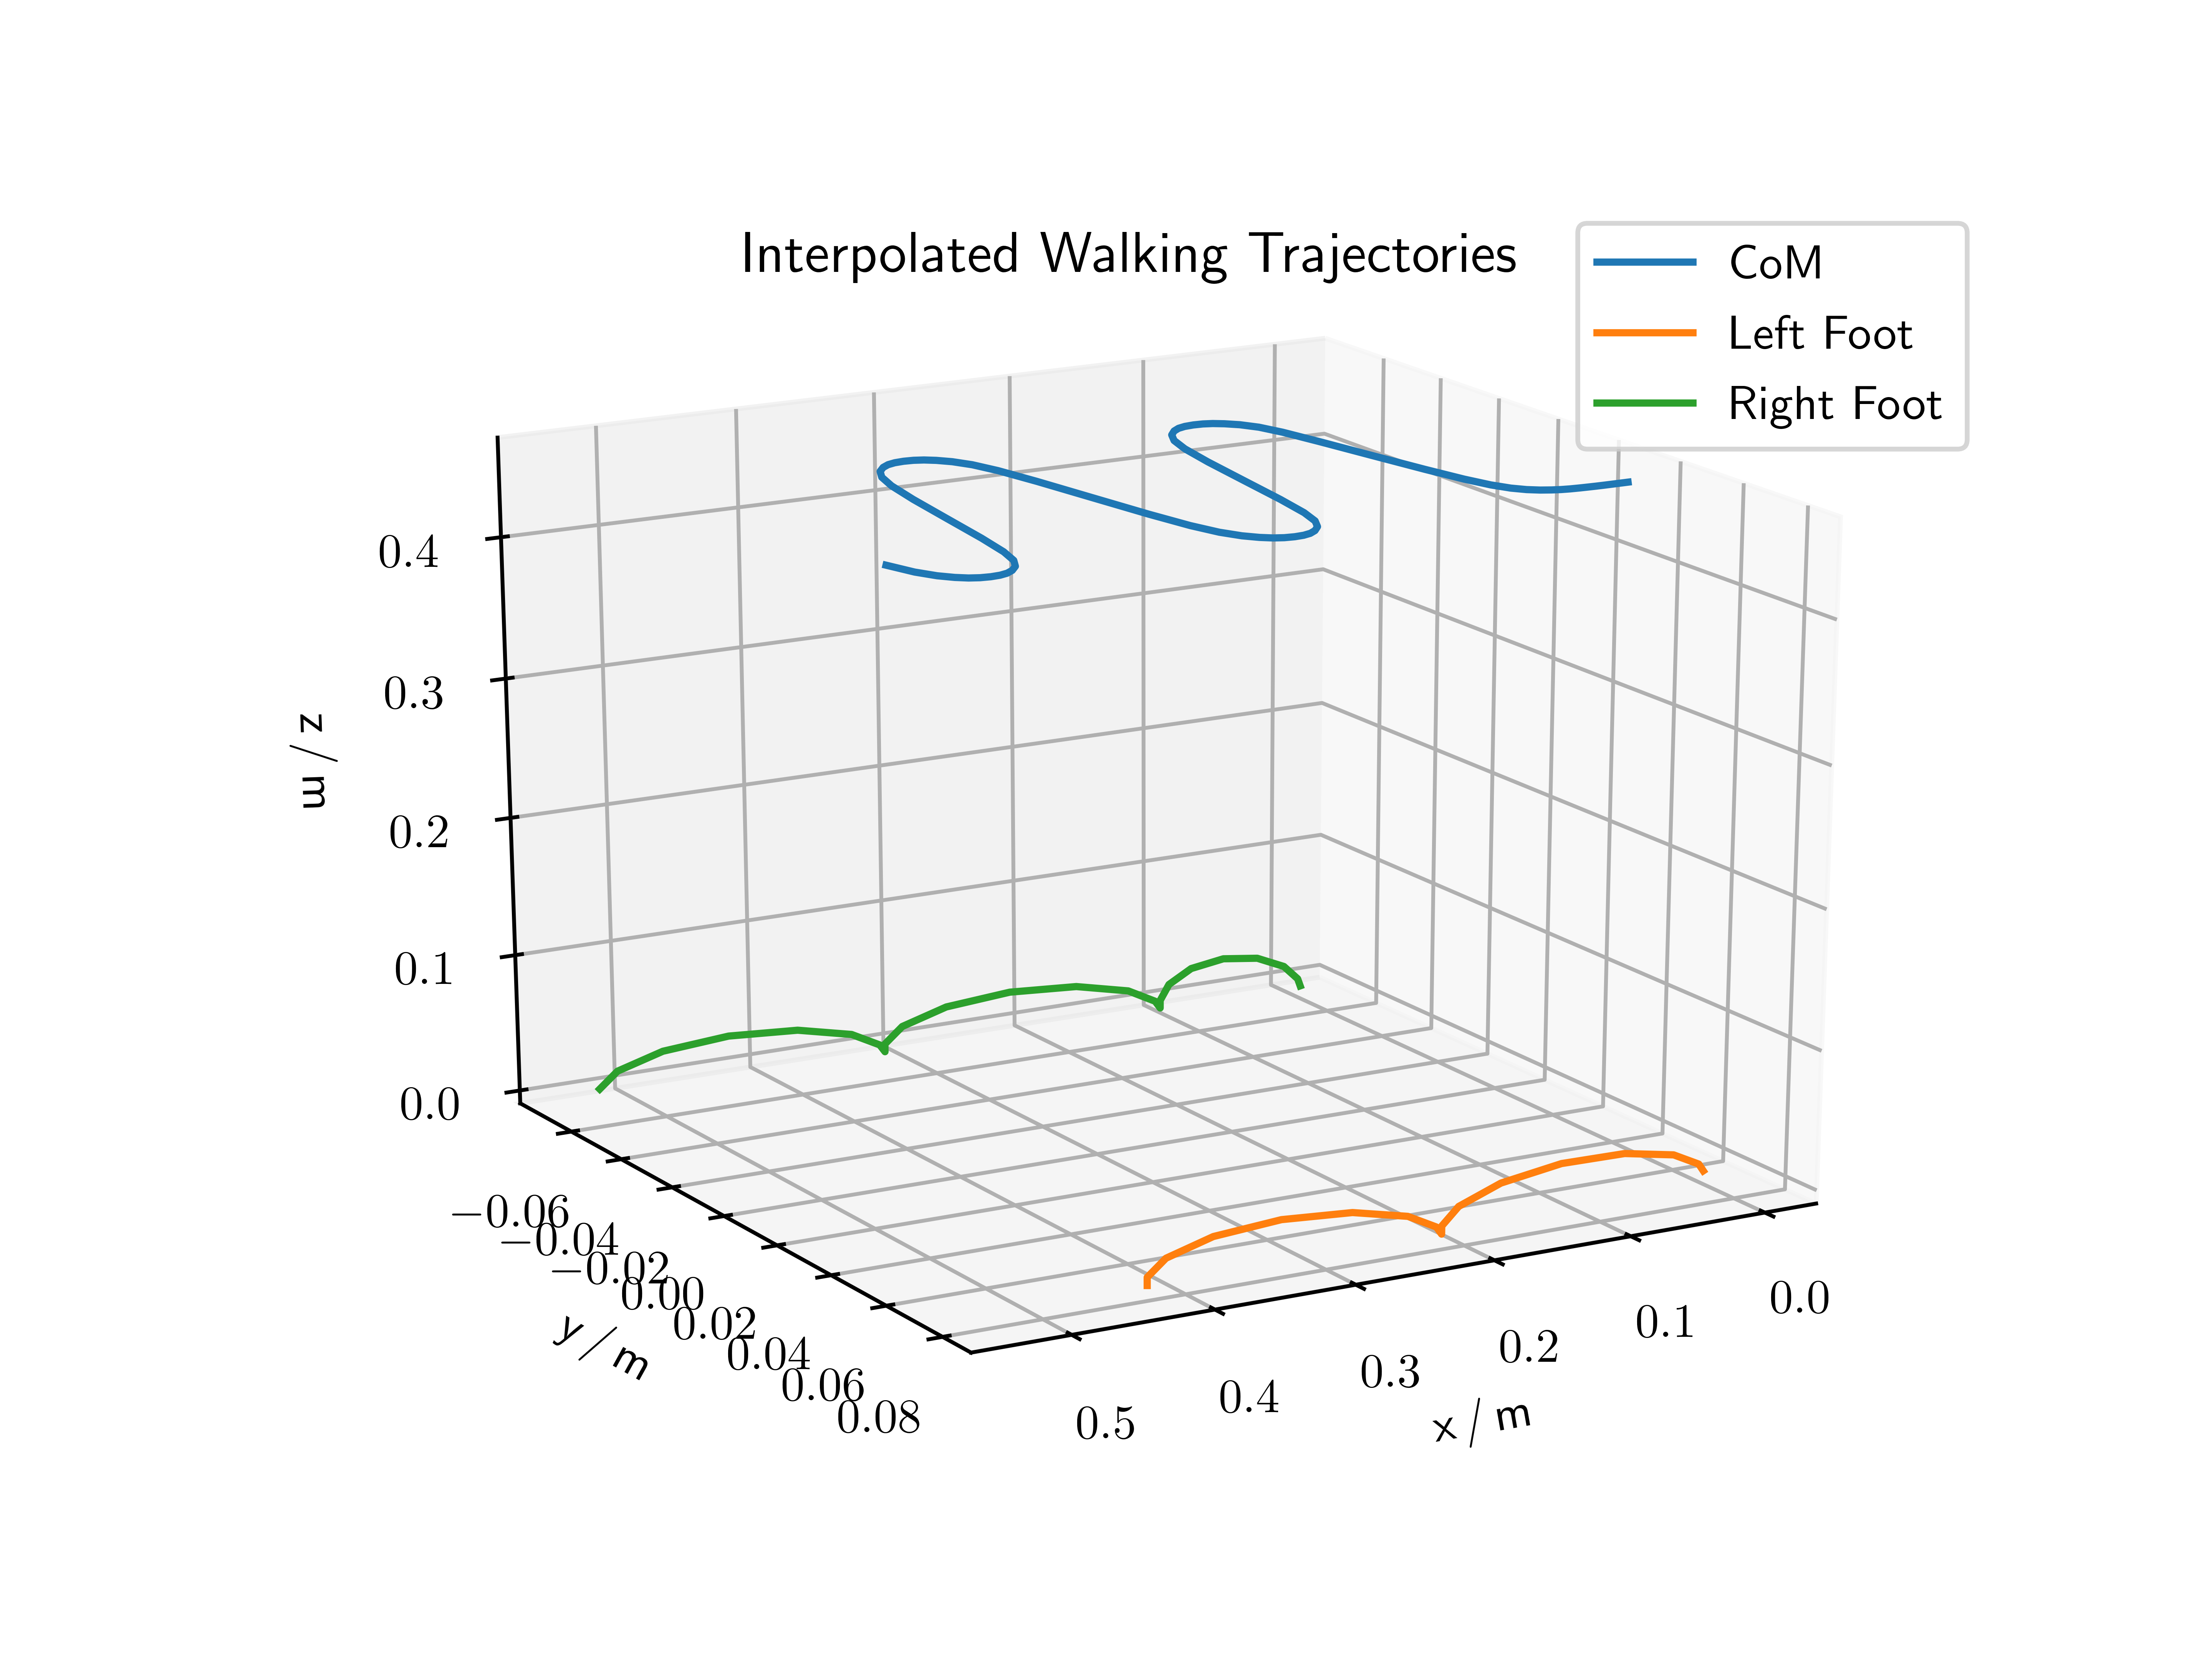
\includegraphics[scale=.4]{chapters/03_background/img/interpolated_results.png}}
	\caption{Uninterpolated trajectories (a), as obtained from the nonlinear model predictive control, and interpolated trajectories (b) for the feet and the center of mass.}
	\label{fig::313_ip}
\end{figure}
\subsubsection{Interpolating the Feet Trajectories}
Any trajectory can in principal be approximated by a polynomial function. For our purposes, we want to approximate positions $p$ as they evolve over time $t$, and further obtain the corresponding velocities $\dot{p}$ and accelerations $\ddot{p}$ (equations \ref{eq::313_pos_poly} - \ref{eq::313_acc_poly}).  
\begin{align}
	p(t) &= \sum_{i = 0}^{N}a_it^i 
	\label{eq::313_pos_poly}\\
	\dot{p}(t) &= \sum_{i = 1}^{N}ia_it^{(i-1)} 
	\label{eq::313_vel_poly}\\
	\ddot{p}(t) &= \sum_{i = 2}^{N}i(i-1)a_it^{(i-2)}
	\label{eq::313_acc_poly}
\end{align}
The coefficients $a_i$ of the polynomials can be chosen such that certain boundary conditions $\bm{b}$ are satisfied. For the lift-off and the drop-down of the robot's feet, these boundary conditions must satisfy a zero initial velocity $\dot{z}_\text{init}$ and a zero end velocity $\dot{z}_\text{end}$, as well as a zero initial height $z_\text{init}$ and a zero end height $z_\text{end}$, and a maximum step height $z_{T/2}$ in between, or else they will hit the ground in an unbalanced way. These conditions are listed below, where each height $z(t)$ and each velocity $\dot{z}(t)$ is written in terms of a polynomial, just as in equations \ref{eq::313_pos_poly} and \ref{eq::313_vel_poly}, respectively. 
\begin{align}
	z(t = 0) &= z_\text{init} = 0
	\label{eq::313_z_bound_1} \\
	\dot{z}(t = 0) &= \dot{z}_\text{init} = 0 \\
	z(t = \frac{T}{2}) &= z_{T/2}\\  
	z(t = T) &= z_\text{end} = 0 \\
	\dot{z}(t = T) &= \dot{z}_\text{end} = 0 
	\label{eq::313_z_bound_5}
\end{align}
To satisfy 5 boundary conditions, it is required to have a polynomial of 4th order with 5 coefficients $a_{z,i}$ in total. In matrix formulation we can express equations \ref{eq::313_z_bound_1} - \ref{eq::313_z_bound_5} as follows
\begin{align}
	\bm{M}_z\bm{a}_z &= \bm{b}_z \\
	\begin{pmatrix}
		1 & 0 & 0              & 0              & 0 \\
		0 & 1 & 0              & 0              & 0 \\
		1 & \left(\frac{T}{2}\right)        & \left(\frac{T}{2}\right)^2  & \left(\frac{T}{2}\right)^3 & \left(\frac{T}{2}\right)^4 \\
		1 & T & T^2            & T^3            & T^4 \\
		0 & 1 & 2T             & 3T^2           & 4T^3 
	\end{pmatrix}
	\begin{pmatrix}
		a_{z,0} \\
		a_{z,1} \\
		a_{z,2} \\
		a_{z,3} \\
		a_{z,4}
	\end{pmatrix} &=
	\begin{pmatrix}
		z_\text{init} \\
		\dot{z}_\text{init} \\
		z_{T/2} \\
		z_\text{end}\\
		\dot{z}_\text{end}
	\end{pmatrix}.
\end{align}
Inversion then yields
\begin{align}
	\bm{a}_z&=\bm{M}_z^{-1}\bm{b}_z \\
	\begin{pmatrix}
		a_{z,0} \\
		a_{z,1} \\
		a_{z,2} \\
		a_{z,3} \\
		a_{z,4}
	\end{pmatrix} &=
	\begin{pmatrix}
		1 & 0 & 0 & 0 & 0 \\
		0 & 1 & 0 & 0 & 0 \\
		-\frac{11}{T^2} & -\frac{4}{T} & \frac{16}{T^2} & -\frac{5}{T^2} & \frac{1}{T} \\
		\frac{18}{T^3} & \frac{5}{T^2} & -\frac{32}{T^3} & \frac{14}{T^3} & -\frac{3}{T^2} \\
		-\frac{8}{T^4} & -\frac{2}{T^3} & \frac{16}{T^4} & -\frac{8}{T^4} & \frac{2}{T^3}
	\end{pmatrix}
	\begin{pmatrix}
		z_\text{init} \\
		\dot{z}_\text{init} \\
		z_{T/2} \\
		z_\text{end}\\
		\dot{z}_\text{end}
	\end{pmatrix}.
\end{align}
The obtained coefficients $a_i$ are then used to compute the height of each foot during a single support phase (\href{https://github.com/mhubii/nmpc_pattern_generator/blob/c82c64a28da7527e75442764f585bd50a8f61ee9/libs/pattern_generator/src/interpolation.cpp#L779}{link}). The maximum step height $z_{T/2}$ (\href{https://github.com/mhubii/nmpc_pattern_generator/blob/c82c64a28da7527e75442764f585bd50a8f61ee9/libs/pattern_generator/configs.yaml#L22}{link}), and the single support time $T$ (\href{https://github.com/mhubii/nmpc_pattern_generator/blob/c82c64a28da7527e75442764f585bd50a8f61ee9/libs/pattern_generator/configs.yaml#L21}{link}), which is the step time minus the double support time, can be set in the configurations file. For the x-, and the y-positions of the feet, we can define boundary conditions in a similar fashion. In contrary to the computation of the z-position, the x-, and the y-position interpolation of the feet allows for feedback. Therefore, we require additional constraints that satisfy the accelerations as follows
\begin{align}
	x(t = 0) &= x_\text{init} 
	\label{eq::313_x_bound_1}\\
	\dot{x}(t=0) &= \dot{x}_\text{init} \\
	\ddot{x}(t=0) &= \ddot{x}_\text{init} \\
	x(t=T) &= x_\text{end}\\
	\dot{x}(t=T) &= \dot{x}_\text{end} \\
	\ddot{x}(t=T) &= \ddot{x}_\text{end}.
	\label{eq::313_x_bound_6}
\end{align}
Again, we can rewrite equations \ref{eq::313_x_bound_1} - \ref{eq::313_x_bound_6} in matrix formulation
\begin{align}
	\bm{M}_x\bm{a}_x &= \bm{b}_x \\
	\begin{pmatrix}
		1 & 0 & 0 & 0 & 0 & 0 \\
		0 & 1 & 0 & 0 & 0 & 0 \\
		0 & 0 & 2 & 0 & 0 & 0 \\
		1 & T & T^2 & T^3 & T^4 & T^5 \\
		0 & 1 & 2 T & 3 T^2 & 4 T^3 & 5 T^4 \\
		0 & 0 & 2 & 6 T & 12 T^2 & 20 T^3
	\end{pmatrix}
	\begin{pmatrix}
		a_{x,0} \\
		a_{x,1} \\
		a_{x,2} \\
		a_{x,3} \\
		a_{x,4} \\
		a_{x,5}
	\end{pmatrix} &=
	\begin{pmatrix}
		x_\text{init} \\
		\dot{x}_\text{init} \\
		\ddot{x}_\text{init} \\
		x_\text{end} \\
		\dot{x}_\text{end} \\
		\ddot{x}_\text{end} 
	\end{pmatrix},
\end{align}
and inversion yields the polynomial's coefficients $a_{x,i}$
\begin{align}
	\bm{a}_x &= \bm{M}_x^{-1}\bm{b}_x \\
	\begin{pmatrix}
		a_{x,0} \\
		a_{x,1} \\
		a_{x,2} \\
		a_{x,3} \\
		a_{x,4} \\
		a_{x,5}
	\end{pmatrix} &= 
	\frac{1}{2}
	\begin{pmatrix}
		2 & 0 & 0 & 0 & 0 & 0 \\
		0 & 2 & 0 & 0 & 0 & 0 \\
		0 & 0 & 1 & 0 & 0 & 0 \\
		-\frac{20}{T^3} & -\frac{12}{T^2} & -\frac{3}{T} & \frac{20}{T^3} & -\frac{8}{T^2} & \frac{1}{T} \\
		\frac{30}{T^4} & \frac{16}{T^3} & \frac{3}{T^2} & -\frac{30}{T^4} & \frac{14}{T^3} & -\frac{2}{T^2} \\
		-\frac{12}{T^5} & -\frac{6}{T^4} & -\frac{1}{T^3} & \frac{12}{T^5} & -\frac{6}{T^4} & \frac{1}{T^3} \\
	\end{pmatrix}
	\begin{pmatrix}
		x_\text{init} \\
		\dot{x}_\text{init} \\
		\ddot{x}_\text{init} \\
		x_\text{end} \\
		\dot{x}_\text{end} \\
		\ddot{x}_\text{end} 
	\end{pmatrix}.
\end{align}
The exact same formalism is used to interpolate the foot's y-position during single support phase (\href{https://github.com/mhubii/nmpc_pattern_generator/blob/c82c64a28da7527e75442764f585bd50a8f61ee9/libs/pattern_generator/src/interpolation.cpp#L806}{link}). In contrast to the interpolation of the feet's positions, the center of mass positions will be extrapolated under the introduced assumption of a linear inverted pendulum. The method will be shortly explained in the following paragraph - Interpolating the Center of Mass Trajectories.
\subsubsection{Interpolating the Center of Mass Trajectories}
The center of mass trajectories can now simply be adjusted to the temporal resolution of the feet trajectories by applying the linear time stepping scheme from equation \ref{eq::321_ltss} with an adjusted temporal resolution $T$. An iterative application (\href{https://github.com/mhubii/nmpc_pattern_generator/blob/5a213044c927dc6aac9f7e32ce1e5fb472cd67bb/libs/pattern_generator/src/interpolation.cpp#L776}{link}) of these matrices then yields the desired interpolation. The only requirement left to get our robot to walk is now the transformation of trajectories in Cartesian space to trajectories within the joint space, which will be resolved in the following chapter - Kinematics.   % interpolation
  \subsection{Kinematics}
\label{sec::314_k}
\subsubsection{Forward Kinematics}
\label{sec::3141_fk}
\subsubsection{Inverse Kinematics}
\label{sec::3142_ik}   % kinematics
  
  \section{Machine Learning}  
\label{sec::32_ml}
   % short overview of machine learning
  \subsection{Behavioral Cloning}
\label{sec::321_bc}   % behavioral cloning
  \subsection{Reinforcement Learning}
\label{sec::322_rl}
   % reinforcement learning
  \subsection{Image Processing}
In the previous sections we have learned about two different approaches to train neural nets on solving certain tasks. Although we came to understand that the complexity of the task to be solved correlates strongly with the amount of data at hand, there exist domains from which it is undeniably easier to do so. To equip a neural net with some sort of prior knowledge by switching the domain may therefore not only be highly desirable but sometimes also needed if the amount or quality of data is not sufficient. One domain which is of special interest when it comes to interacting in a three dimensional environment is a domain that represents depth information. If there are any, it may sometimes be possible to extract this kind of prior knowledge from a depth camera. As for this work, we need to rely on stereo cameras and powerful algorithms that allow us to compute depth images in real time. The algorithm that helps us to do so, in terms of the extraction of weighted least squares disparity maps, will be presented in the following paragraph - Depth Map Extraction.
\subsubsection{Depth Map Extraction}
As already pointed out, the depth map is generated from stereo camera images by a technique called stereo matching \cite{hamzah2010sum}. This method works best for  
\begin{figure}[h]
	\centering
	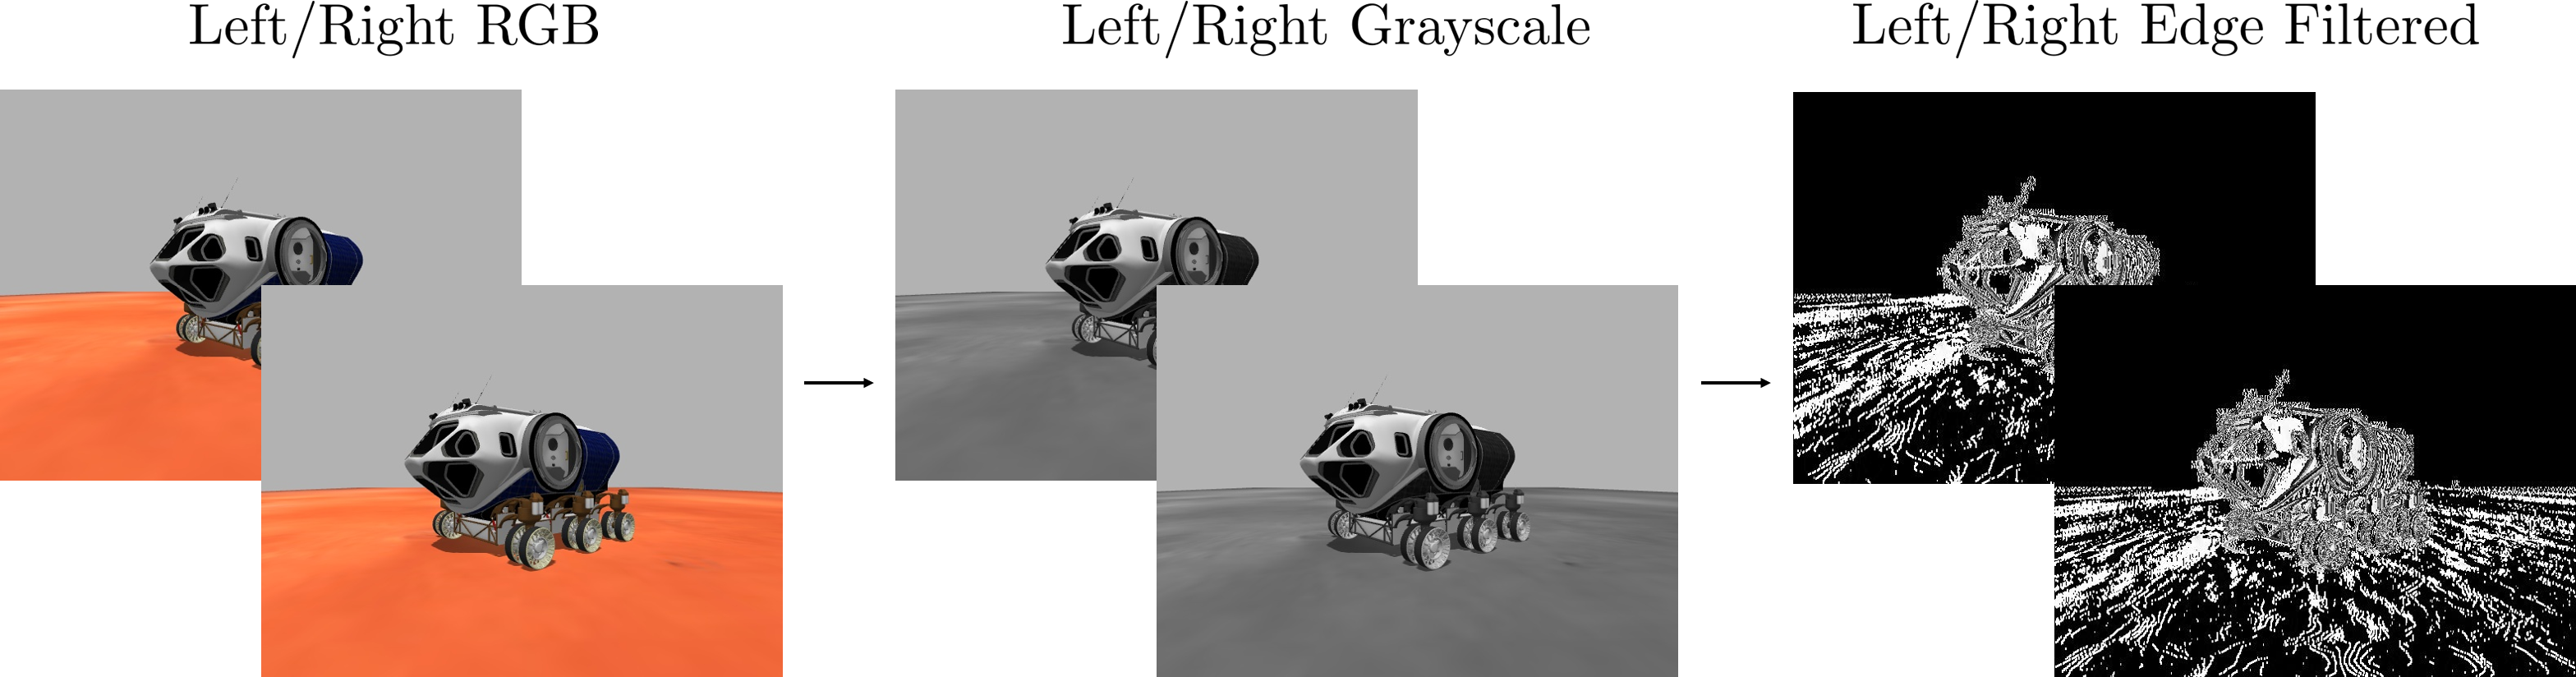
\includegraphics[scale=.25]{chapters/03_background/img/image_preprocessing.png}
	\caption{}
	\label{fig::323_image_preprocessing}
\end{figure}
\begin{figure}[h]
	\centering
	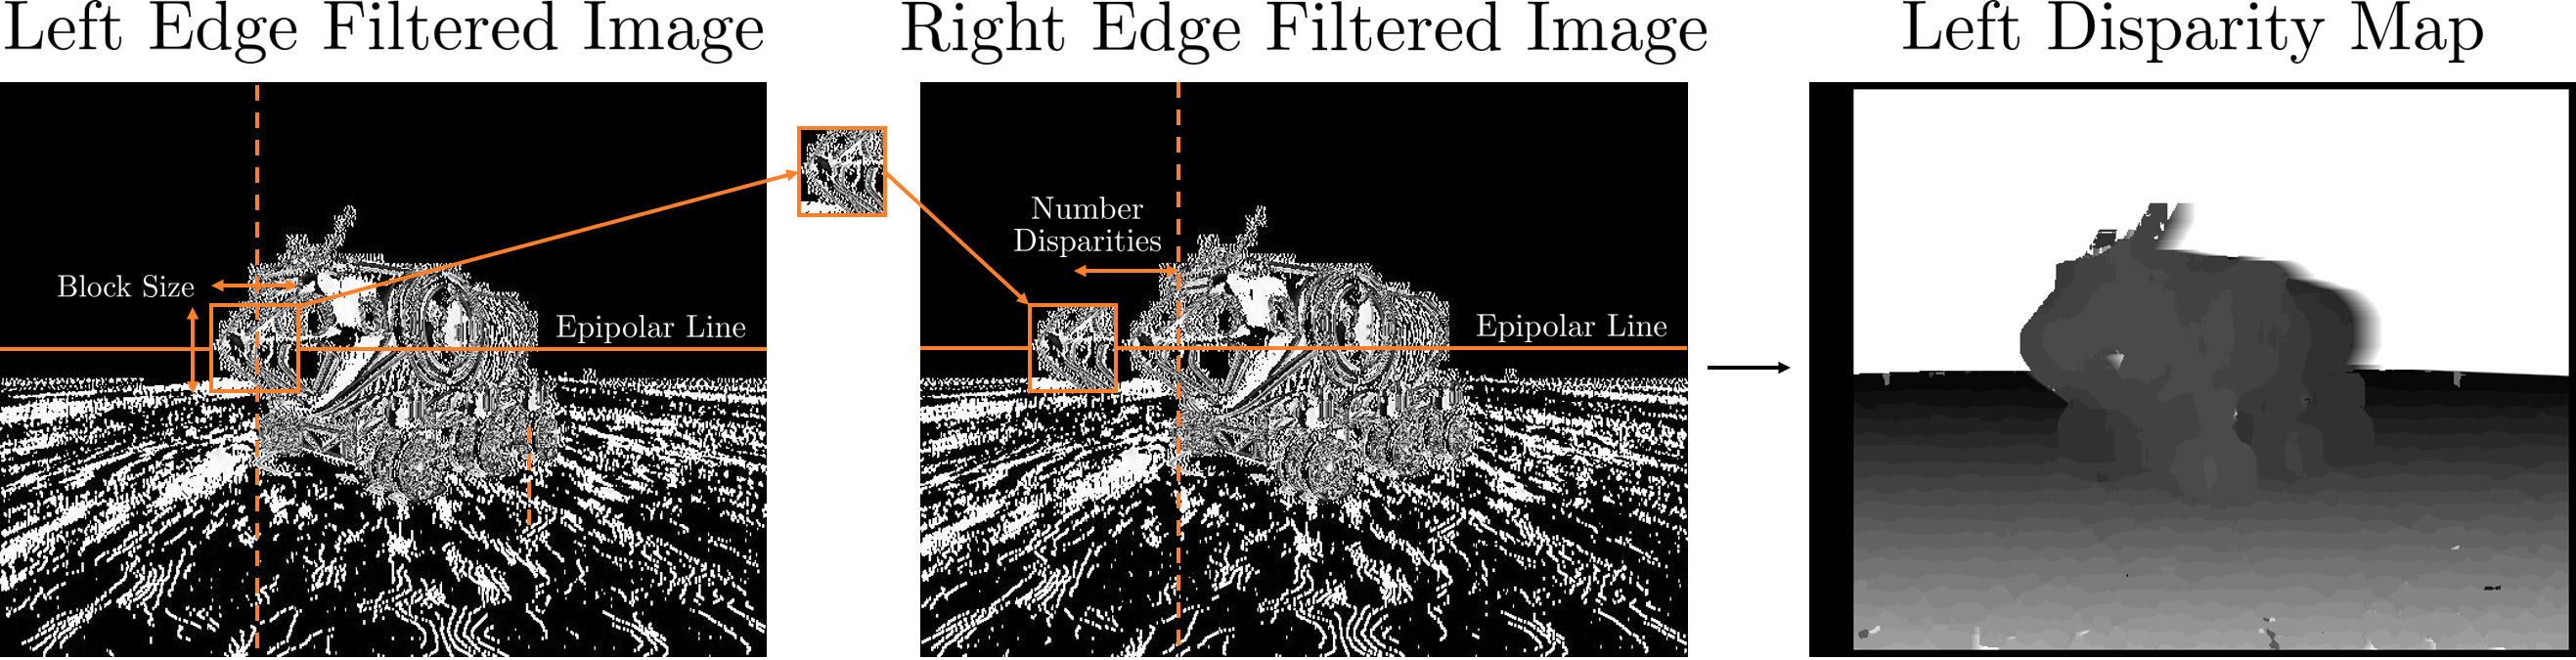
\includegraphics[scale=.3]{chapters/03_background/img/left_disparity_map.png}
	\caption{}
	\label{fig::323_left_disparity_map}
\end{figure}
\cite{sobel2014an}   sobel\\
\cite{hamzah2010sum} stereo matching\\
\cite{egnal2004stereo} left right consistency\\
\cite{min2014fast}   wls\\
\cite{tomasi1998bilateral} bilateral
\\\\
As a requirement for the algorithm to work properly, it is important to calibrate the robot's cameras. Therefore, the next chapter - Mono and Stereo Camera Calibration, will explain in detail why, and how to calibrate cameras.
\subsubsection{Mono and Stereo Camera Calibration}   % image processing
   
  \chapter{Methods}
  \section{Software}
  %\input{chapters/04_methods/01_eig}     % eigen
  %\input{chapters/04_methods/02_qp}      % qpoases
  %\input{chapters/04_methods/03_rbdl}    % rbdl
  %\input{chapters/04_methods/04_yarp}    % yarp
  %\input{chapters/04_methods/05_pyt}     % pytorch
  %\input{chapters/04_methods/06_cv}      % opencv
  
  \section{Implementation}  
   
  \chapter{Experiments}
  
  \section{User Controlled Walking}
  
  \section{Autonomous Walking}

  \chapter{Conclusion}

  \part{Appendix}
  \begin{appendix}
    \chapter{Lists}
    \listoffigures
    \listoftables
    \bibliographystyle{unsrt}
    \bibliography{chapters/07_appendix/references}
    \setlength{\parindent}{0em}

Erkl\"{a}rung:\par
\vspace{3\baselineskip}
Ich versichere, dass ich diese Arbeit selbstst\"{a}ndig verfasst habe und keine
anderen als die angegebenen Quellen und Hilfsmittel benutzt habe.\par
\vspace{5\baselineskip}
Heidelberg, den (Datum)\hspace{3cm}\dotfill

  \end{appendix}
\end{document}
